\section{题目1(学时2):}
创建一个由6个结点的单向链表,实现增加、删除、查找、移动、显示结点的基本功能。
\\

\lstinputlisting[language=protobuf2, style=protobuf,caption={%
题目1}]{search1.proto}
\section{运行结果}
\begin{figure}[ht]

    \centering
    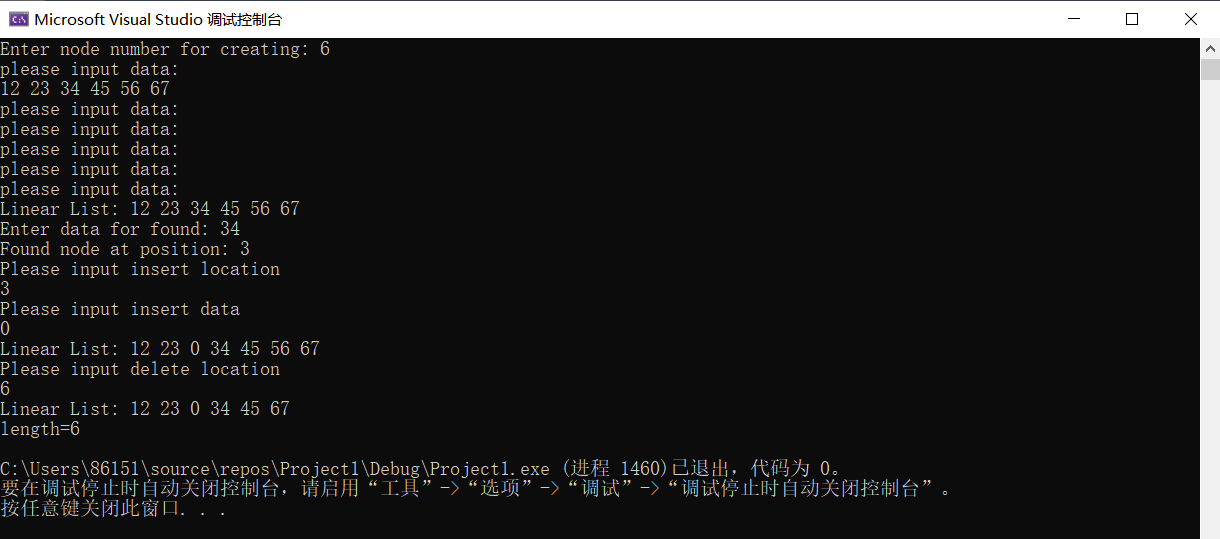
\includegraphics[scale=0.6]{图片1.png}
    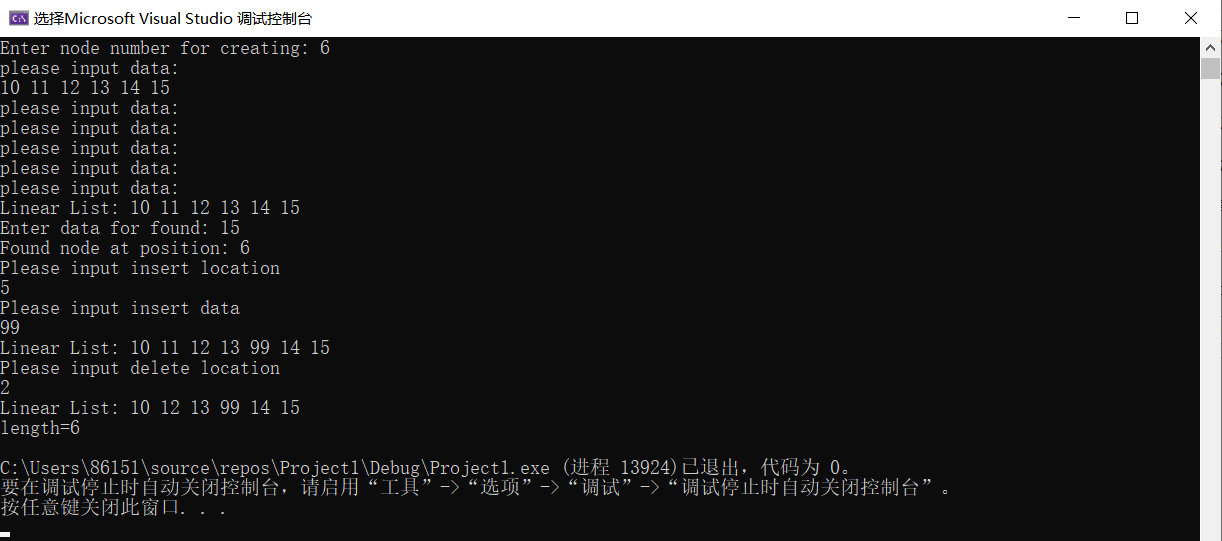
\includegraphics[scale=0.6]{图片2.png}
    \caption{题目1运行结果}
    \label{fig:label}
    \end{figure}
\section{题目2 :字符逆转(学时:2)}
从键盘读入一个字符串,把它存入一个链表(每个结点存储1个字符),并按相反的次序将字符串输出到显示屏。
\lstinputlisting[language=protobuf2, style=protobuf,caption={%
题目2 :字符逆转(学时:2)}]{search1 copy.proto}


\section{题目2运行结果}
\begin{figure}[ht]

    \centering
    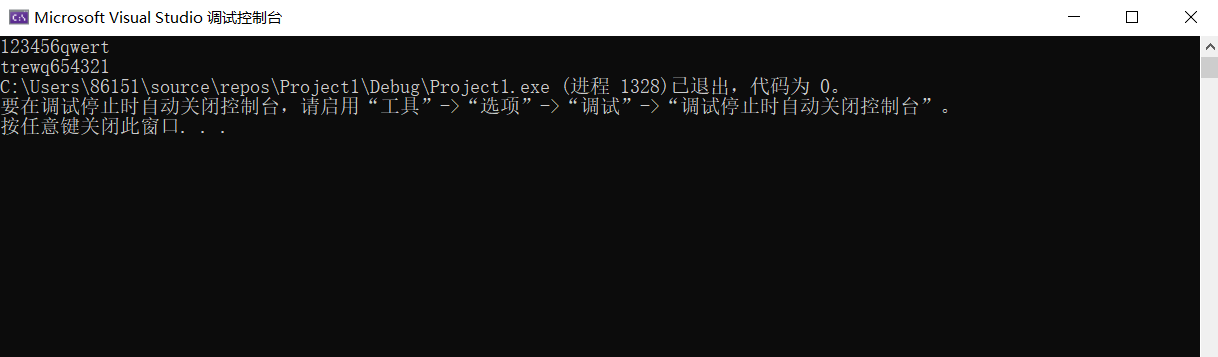
\includegraphics[scale=0.6]{图片3.png}
    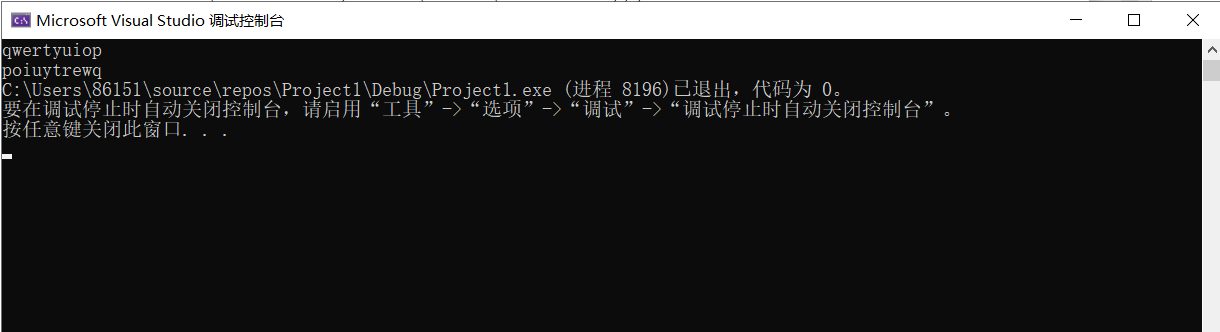
\includegraphics[scale=0.6]{图片4.png}
    \caption{题目2运行结果}
    \label{fig:label}
    \end{figure}


